% CHAPTER 3


In order to measure the surface stress of soft matter at varying strains, it is necessary to have a device capable of controllably stretching and holding silicone sheets at a constant strain equibiaxially. To achieve this, we built a stretching apparatus based off of the work of Na \cite{na2008time} and Xu \cite{xu2017direct}. Full details of the stretching apparatus can be found in appendix A. 

Aluminum was chosen as the base material because of its sturdy yet malleable nature, making it an excellent material with which to mill. Acrylic was considered, but was not chosen because of its brittle nature; we were concerned about cracking when drilling the UNF threads connecting to the Luer-lock syringe.

Geometrically, the stretching apparatus is constructed of two cylinders connected at the base to create a channel between them. The top of each ring is flat, apart from a slight chamfer to reduce the risk of ripping the sheet needed to be stretched. Each ring is then coated in Dow Corning vacuum grease to make a seal. It is critical that the inner ring has an ample amount of grease so that when a vacuum is pulled in the channel, the sheet will stretch from the center outwards  and not from the edges inwards.  

The stretched sheet is laid over the gelled apparatus and fixed in place using a 48.7mm diameter by 1.6mm thick rubber O-ring. A removable plastic ring is then placed on top of the o-ring and clamped down using a tension clamp attached to a fitted plastic base. The plastic ring is constructed from an engineering plastic that came from a similar but malfunctioning device used by our colleagues at ETH Zürich. The tension provided by the o-ring and clamp ensure that a solid vacuum is kept and the edges of the sheet are minimally stretched into the trough. The outer ring could easily be laser cut from a plastic or milled out of aluminum if desired. 

To pull a vacuum, a 1/4-28 UNF to female Luer connects the apparatus to a plastic 100ml Luer-lock syringe. We found a more consistent stretch was held by lining the inner walls of the syringe in more Dow Corning vacuum grease. The UNF to female luer connector is stainless steal, and \emph{sealed into place with epoxy resin. Note: I haven't done this yet 190322, but I think I should. But make sure to get the o-ring size first...and i think one size smaller would actually work better}
coated with Dow Corning vacuum grease. The inclusion of a small o-ring between the UNF threads and the cylindrical base proved critical in holding vacuum for sustained periods of time.

The vacuum pull was controlled by a Harvard Apparatus Elite 11 Syringe Pump. Stretching was found to work best at maximum withdrawal rate. Our stretching apparatus has sustained a constant equibiaxial stretch at 36\% strain for as long as 5 hours. Maximum strain percentage and during of maintained stretch is yet to be fully tested.


\section{Calibration}
Originally, we intended to calibrate the strain value induced by the vacuum to the extent that we could predict the induced strain based on the amount of air withdrawn from the stretching apparatus. We withdrew air from the syringe and measured the movement of $~10\mu m$ beads using a 10x air lens on our Nikon confocal microscope. Using the transmission detector allowed us to image the surface of our material with a wide field of view. Strain percentage was calculated using MATLAB code written by Ross (masterGUI then strain Cal). \emph{Note, might come back, cut this and move to next subsubsection. I have it doubled for now.}

There are several obstacles in calibrating the induced strain. First, the stretching apparatus works best when a large strain is applied. Applying small strains one after another works but there is a threshold to induce stretch. No stretching change is visible if less than 2ml is withdrawn from the cylinder per increment. Thus, there is a limited resolution to our calibration data, which would not be a problem if the strain was linear. However, preliminary measurements indicated that the applied strain was nonlinear. This agrees with the with previous results \cite{na2008time} obtained using a similar device. \emph{note to self, double check this is where that graph I'm thinking about actually showed up}. Lastly, the greatest problem with calibrating strain is that we change substrates often. Even if we were to use the same exact sample, by removing it and setting up the device again, there is no way to standardize a zero-applied strain point. To prepare the stretching device, the sample is placed over the opening and a rubber o-ring is placed around the sample to help affix it in place. The sample must then be stretched and wiggled around slightly to remove any snags that could jeopardize the vacuum's efficacy. This means that every time a new sample is prepared, it is in an unknown and unique state of induced strain. It could even have less than zero strain if the sample is loose in large center opening \emph{Think of better name for this.} 

 It was thus determined best to measure strain every time we applied a new strain to the silicone substrate and compare it to the substrate's original state. This also assured us that we knew the correct strain value to a higher precision for any given data set. Additionally, with the pleasantly unexpected ability to hold strains exceeding 30\%, the $2\mu$m resolution  limit became superfluous in seeking to measure $\Upsilon(\epsilon)$.
 
\subsubsection{Measuring Strain}
Things to talk about here:\\
- Lens and TD settings \checkmark \\
- Tracking code, including the generated images \\
- The tifs including the overlay I used in the APS talk \\

To determine the induced strain, we maximized the field of view. This allows us to see how more more spheres are shifting, and thus gives a more accurate estimate of induced strain. As such, we decided to switch to the bright-field and measure how the spheres were shifting when stretched. We used a 10x air lens in conjunction with the transmission detector on our Nikon Confocal. We adjust the settings to give decent contrast, but it is more important to have the spheres in focus. For our Nikon this usually means setting the Power (HV) to 80. \emph{again...what's HV stand for?} Each sphere reflects light, and it is this reflection that our particle locating software tracks after some image processing. An example image is located below, next to the same image after adjusting the contrast to help our tracking software with particle locating: \emph{um...how well is the image on the right going to print...? Also, the centering is weird for this}

  \begin{figure}[h]
  		\label{fig:TDpreandpost}
  	\begin{tabular}{cc}
  		
\includegraphics[width= .48\linewidth]{Chapters/Figures/1xzoom_constellation_zeroStrain.png} & 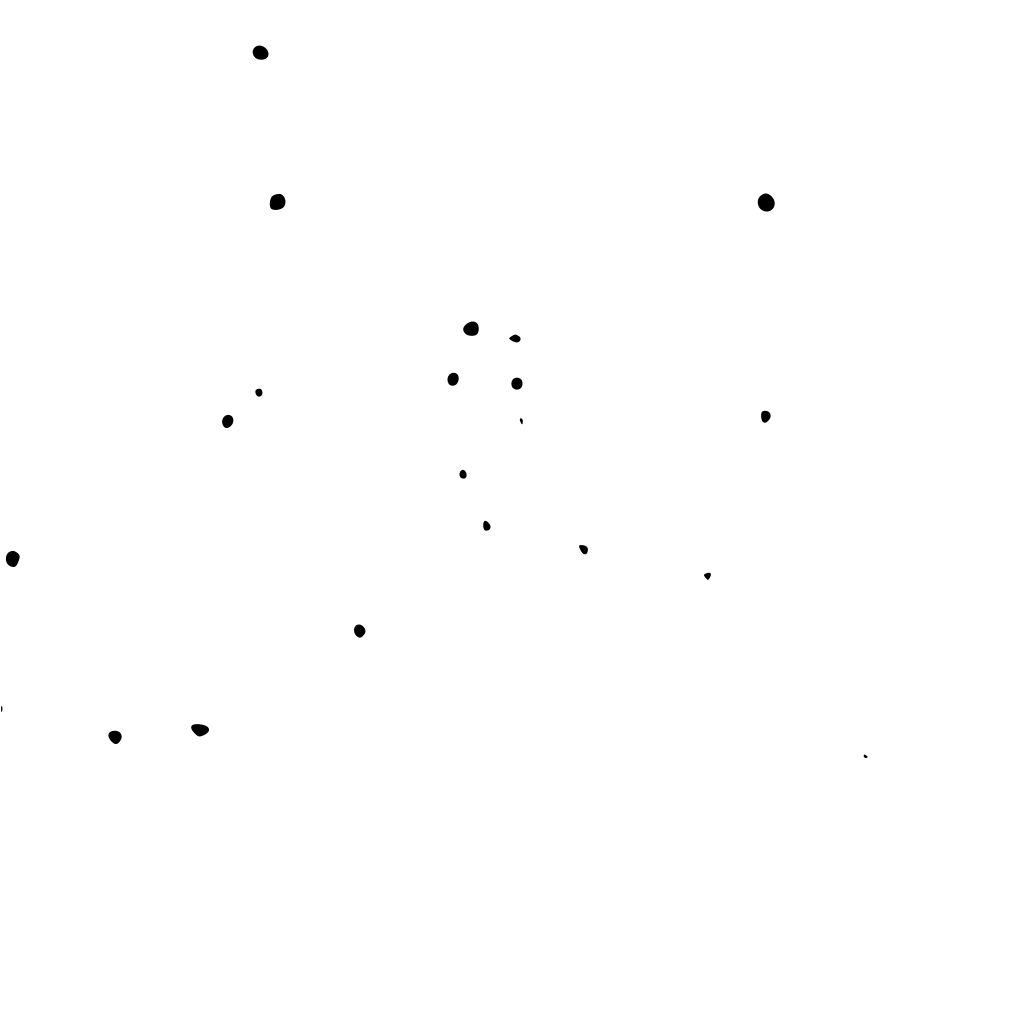
\includegraphics[width= .48\linewidth]{Chapters/Figures/1xzoom_constellation_zeroStrain_supercontrast.png}\\
  		Fig. A & Fig. B
  			\end{tabular}
  \caption[Bright-field pre and post image processing]{Figure A shows the calibration constellation before any strain is applied. Fig. B shows the same image after processing. Only the sphere reflections remain.}
\end{figure}

To track how the substrate stretches, we first find a centrally located group of spheres, or ``constellation.'' A good constellation is one that easily identifiable for relocation and tracking purposes, and one that has many discrete points in the field of view - i.e. there are plenty of non-overlapping spheres. \emph{It is an added bonus to find 4 spheres perpendicularly located, such that they form the tips of cross.} Though not necessarily, this is useful for a preliminary strain calculation using the built in measuring functions on the Microscope's software. It is nice to track the progression of stretching and ensure the substrate is not preferentially stretching in on direction; this could indicate the substrate is caught in the apparatus. Not only does this ruin the symmetry assumptions being made for our calculation, but it could lead to the substrate tearing if more strain is being applied than expected.

To evacuate the cylinder, we use the the Harvard Apparatus\texttrademark \ Elite Pro Syringe Pump with a 50ml Luerlock syringe. Before beginning any stretching, we withdraw a few ml of air to ensure the substrate is flat and not sagging. At this point we take a picture of the brightfield and call it the ``zero applied strain'' image. We compare all stretched data to this image in order to determine the induced strain. Because of the geometry of the stretching apparatus, along with the way the silicone cures, it is difficult \emph{impossible??} to determine the true strain of the silicone. However, we are most interested in the slope of the $\Upsilon$ vs. $\epsilon$ curve, $\Lambda$, so this is not vitally important.

The induced strain is a tensor of rank two. \emph{If I'm bored and have time, I'd like to add an appendix to talk about this tensor. I think that would be the best way for me to really understand it. That graphic in the book hasn't really stuck with me} Because we are stretching the substrate equally in all directions, we can just look at the magnitude of the tensor and treat the strain as a scalar.     

 
\begin{figure}[h!]
	\centering
	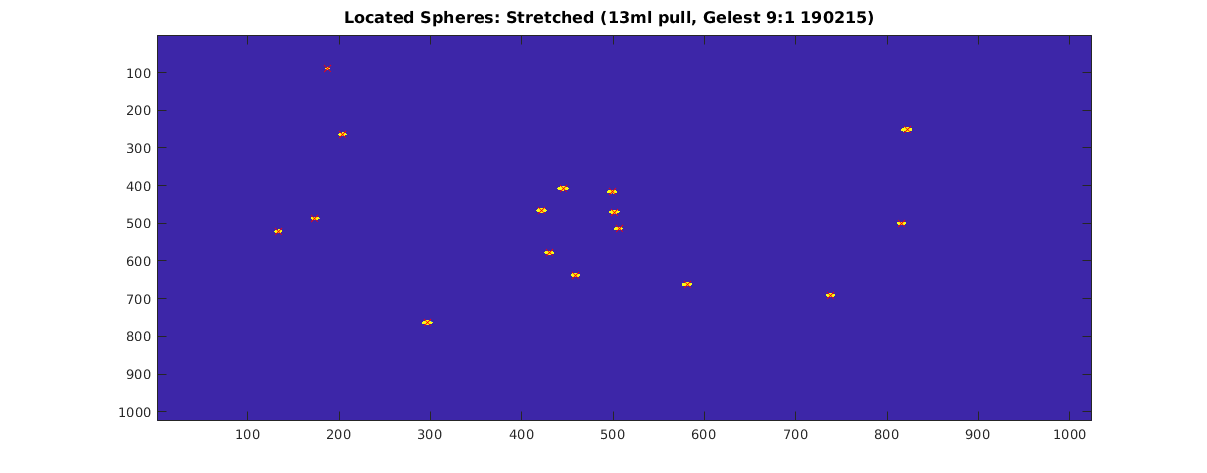
\includegraphics[width=0.7\linewidth]{Chapters/Figures/13ml_stretched_2D_located}
	\caption[Unstretched]{}
	\label{fig:13mlstretched2dlocated}
\end{figure}

\begin{figure}[h!]
	\centering
	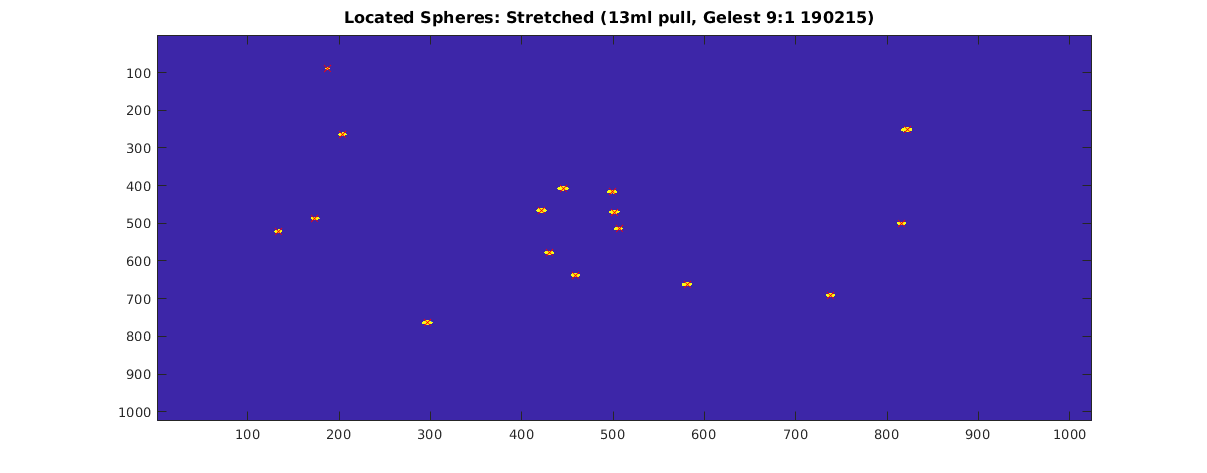
\includegraphics[width=0.7\linewidth]{Chapters/Figures/13ml_stretched_2D_located}
	\caption[Stretched]{These are placeholders for now. I don't really like how they look and I don't think they're totally necessary. It might be nice to keep them if I can clean them up. Especially if I get some nice stretch data with the new DC}
	\label{fig:13mlstretched2dlocated}
\end{figure}

%